\documentclass{article}
\usepackage[margin=1in]{geometry}
\usepackage{amsmath,amsthm,amssymb}
\usepackage{bbm,enumerate,mathtools}
\usepackage{tikz,pgfplots}
\usepackage{chessboard}
\usepackage[hidelinks]{hyperref}
\usepackage{multicol} % Problem 35

\newenvironment{question}{\begin{trivlist}\item[\textbf{Question.}]}{\end{trivlist}}
\newenvironment{note}{\begin{trivlist}\item[\textbf{Note.}]}{\end{trivlist}}
\newenvironment{references}{\begin{trivlist}\item[\textbf{References.}]}{\end{trivlist}}
\newenvironment{related}{\begin{trivlist}\item[\textbf{Related.}]\end{trivlist}\begin{enumerate}}{\end{enumerate}}


\begin{document}
\rating{1}{2}
Consider all $k$-colorings of an $n \times n$ grid, where each row and column
has $\lfloor n/k \rfloor$ or $\lceil n/k \rceil$ cells with each color.
\begin{figure}[!h]
  \centering
  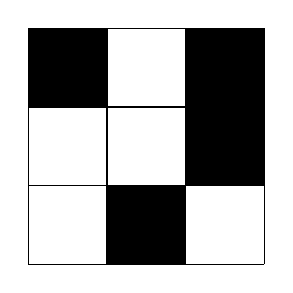
\begin{tikzpicture}
    \fill (0,2) rectangle (1,3);
    \fill (2,2) rectangle (3,3);
    \fill (2,1) rectangle (3,2);
    \fill (1,0) rectangle (2,1);
    \draw (0,0) grid (3,3);
  \end{tikzpicture} \hspace{1cm}
  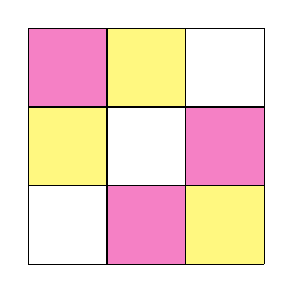
\begin{tikzpicture}
    \fill[magenta!50] (0,2) rectangle (1,3);
    \fill[magenta!50] (2,1) rectangle (3,2);
    \fill[magenta!50] (1,0) rectangle (2,1);
    \fill[yellow!50] (1,2) rectangle (2,3);
    \fill[yellow!50] (0,1) rectangle (1,2);
    \fill[yellow!50] (2,0) rectangle (3,1);
    \draw (0,0) grid (3,3);
  \end{tikzpicture}
  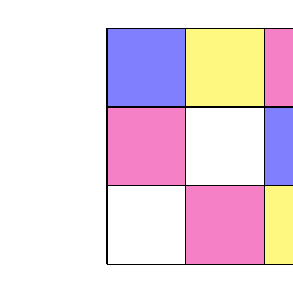
\begin{tikzpicture} \hspace{1cm}
    \fill[blue!50] (0,2) rectangle (1,3);
    \fill[blue!50] (2,1) rectangle (3,2);
    \fill[yellow!50] (1,2) rectangle (2,3);
    \fill[yellow!50] (2,0) rectangle (3,1);
    \fill[magenta!50] (0,1) rectangle (1,2);
    \fill[magenta!50] (1,0) rectangle (2,1);
    \fill[magenta!50] (2,2) rectangle (3,3);
    \draw (0,0) grid (3,3);
  \end{tikzpicture}
  \caption{A valid 2-coloring, 3-coloring, and 4-coloring of an $3 \times 3$ grid.}
\end{figure}

\begin{question}
  How many such $k$-colorings of the $n \times n$ grid?
\end{question}

\begin{related}
  \item What if there also must be a total of
    $\lfloor n^2/k \rfloor$ or $\lceil n^2/k \rceil$ cells of each color?
  \item What if these are counted up to the dihedral action on the square $D_4$?
  \item What if these are counted up to torus action?
  \item What if these are counted up to permutation of the coloring?
  \item Can this generalize to the cube? To a triangular tiling?
\end{related}
\end{document}
